\section*{Deep Neural Networks}

\textbf{Deep Learning}: a class of machine learning methods that use multiple layers of non-linear transformations to learn complex patterns in data.

\begin{itemize}
  \item Extracting high-level, abstract features is a difficult problem in \textbf{representation learning}.
  \item Deep learning  \enquote{solves} it by introducing representations that are expressed in terms of other, simpler representations - allowing computers to build complex concepts out of simpler ones.
  \item Example: in an image classification task, a deep neural network might learn to recognize \textbf{edges} in the first layer, \textbf{edges/contours} in the second layer, and \textbf{object parts} in the third layer.
\end{itemize}

\subsection*{Multi-Layer Perceptron (MLP)}

\begin{itemize}
  \item \textbf{Goal:} Approximate a function $\mathbf{y} = f^*(\mathbf{x})$ by defining a mapping $\mathbf{y} = f(\mathbf{x}; \boldsymbol{\uptheta})$ and learning values of $\boldsymbol{\uptheta}$ which result in best approximation.
  \item Also known as \textbf{feedforward neural network}, because information flows from $\mathbf{x}$ through the intermediate computations used to define $f$ and finally to $\mathbf{y}$. There are \textbf{no feedback connections}.
  \item This forward flow of information is also known as \textbf{forward propagation}. Forward propagation takes place during \textbf{both training and inference phases}.
  \item \textbf{Back-propagation} allows the error information to flow from the output layer backwards through the network, in order to compute the gradients of the loss function with respect to the parameters $\boldsymbol{\uptheta}$ ($\nabla_{\boldsymbol{\uptheta}} J (\boldsymbol{\uptheta})$).
\end{itemize}

\subsection*{Local-Minima Problem}
\begin{itemize}
  \item The loss function $J(\boldsymbol{\uptheta})$ is a non-convex function, which means it can have \textbf{multiple local minima}.
  \item Gradient descent may converge to a local minimum instead of the global minimum.
  \item To mitigate: (i) Random initializations/restarts, (ii) stochasticity (SGD), (iii) momentum, (iv) adaptive optimizers, (v) learning rate schedules, (vi) batch normalization
  \item For large deep nets, most local minima are \textbf{good enough} for practical purposes. \textbf{Saddle points} or \textbf{plateaus} are bigger issues.
\end{itemize}

\subsection*{Pretraining}
  \begin{itemize}
    \item A Model is trained on a large, generic dataset (e.g., ImageNet for vision, large text corpus for NLP).  
    \item \textbf{Goal}: Learn general-purpose features or representations (edges, textures, word embeddings, contextual patterns).  
    \item Usually self-supervised or unsupervised objectives (e.g., masked language modeling, contrastive learning).  
    \item \textbf{Provides a strong initialization} that (i) speeds up convergence and (ii) improves generalization on downstream tasks.
  \end{itemize}

\subsection*{Fine-Tuning}
\begin{itemize}
      \item Start from the pretrained weights and continue training on a smaller, task-specific labeled dataset.  
      \item Often uses a lower learning rate to preserve useful pretrained features while adapting to the new task.  
      \item Can involve:
        \begin{itemize}
          \item \textbf{Full-model tuning:} update all layers.  
          \item \textbf{Partial tuning:} freeze early layers and only train later layers or an added task head.  
          \item \textbf{Adapter modules}: insert lightweight trainable parameters while keeping most weights fixed. (e.g., \textbf{LoRA})
        \end{itemize}
      \item Benefits:
        \begin{itemize}
          \item Requires far \textbf{fewer labeled examples} than training from scratch.  
          \item Achieves \textbf{higher accuracy} and \textbf{faster convergence} on the target task.  
          \item \textbf{Reduces overfitting}, especially when available labeled data is limited.
        \end{itemize}
\end{itemize}

\subsection*{AutoEncoders}
    \textbf{Autoencoder}: A neural network trained to attempt to copy its input to its output. It has a hidden layer $\mathbf{h}$ that describes a code used to represent the input.
\begin{itemize}
  \item Two parts: (i) encoder function ($\mathbf{h} = f(\mathbf{x})$) and (ii) decoder function ($\mathbf{r} = g(\mathbf{h})$).
  \item \textbf{Undercomplete Autoencoder}: $\text{dim}(\mathbf{h}) < \text{dim}(\mathbf{x})$, model learns a compressed representation. Learning process is described as minimizing a loss function $L(\mathbf{x}, g(f(\mathbf{x})))$. This is known as \textbf{reconstruction loss}.
  \item \textbf{Overcomplete Autoencoder}: $\text{dim}(\mathbf{h}) > \text{dim}(\mathbf{x})$, model learns a more complex representation. Usually not useful.
  \item \textbf{Regularized Autoencoders}: Use a loss function that encourages the model to have other properties besides the ability to copy its input to its output. These other properties include: (i) \textbf{sparsity} of the representation, (ii) \textbf{smallness of the derivative} of the representation, and (iii) \textbf{robustness to noise or to missing inputs}

    \begin{itemize}
      \item \textbf{Sparse Autoencoders}: \textbf{Goal:} encourage the model to use only a small number of hidden units to represent the input. Sparsity penalty $\Omega(\mathbf{h})$ on the hidden layer $\mathbf{h}$, in addition to the reconstruction loss: $L(\mathbf{x}, g(f(\mathbf{x}))) + \Omega(\mathbf{h})$.
      \item \textbf{Denoising Autoencoders}: \textbf{Goal:} train the model to reconstruct the original input from a \textbf{corrupted version} of it. \textbf{Loss:} $L(\mathbf{x}, g(f(\tilde{\mathbf{x}})))$, where $\tilde{\mathbf{x}}$ is a noisy version of $\mathbf{x}$.
      \item \textbf{Contractive Autoencoders}: \textbf{Goal:} train the model to learn a representation that does not change much when $\mathbf{x}$ changes slightly. Addition of a penalty term that encourages the model to have small derivatives with respect to the input. \textbf{Loss:} $L(\mathbf{x}, g(f(\mathbf{x}))) + \Omega (\mathbf{h}, \mathbf{x})$ where $\Omega(\mathbf{h}, \mathbf{x}) = \lambda \sum_i || \nabla_{\mathbf{x}} h_i ||^2$.
    \end{itemize}
\end{itemize}

\subsection*{Activation Functions}
An \textbf{activation function} introduces non-linearity into the model, allowing it to learn complex patterns.
\begin{itemize}
  \item Sigmoid: $f(x) = \frac{1}{1 + e^{-x}}$
    \begin{figure}[H]
      \centering
      \vspace{-1em}
      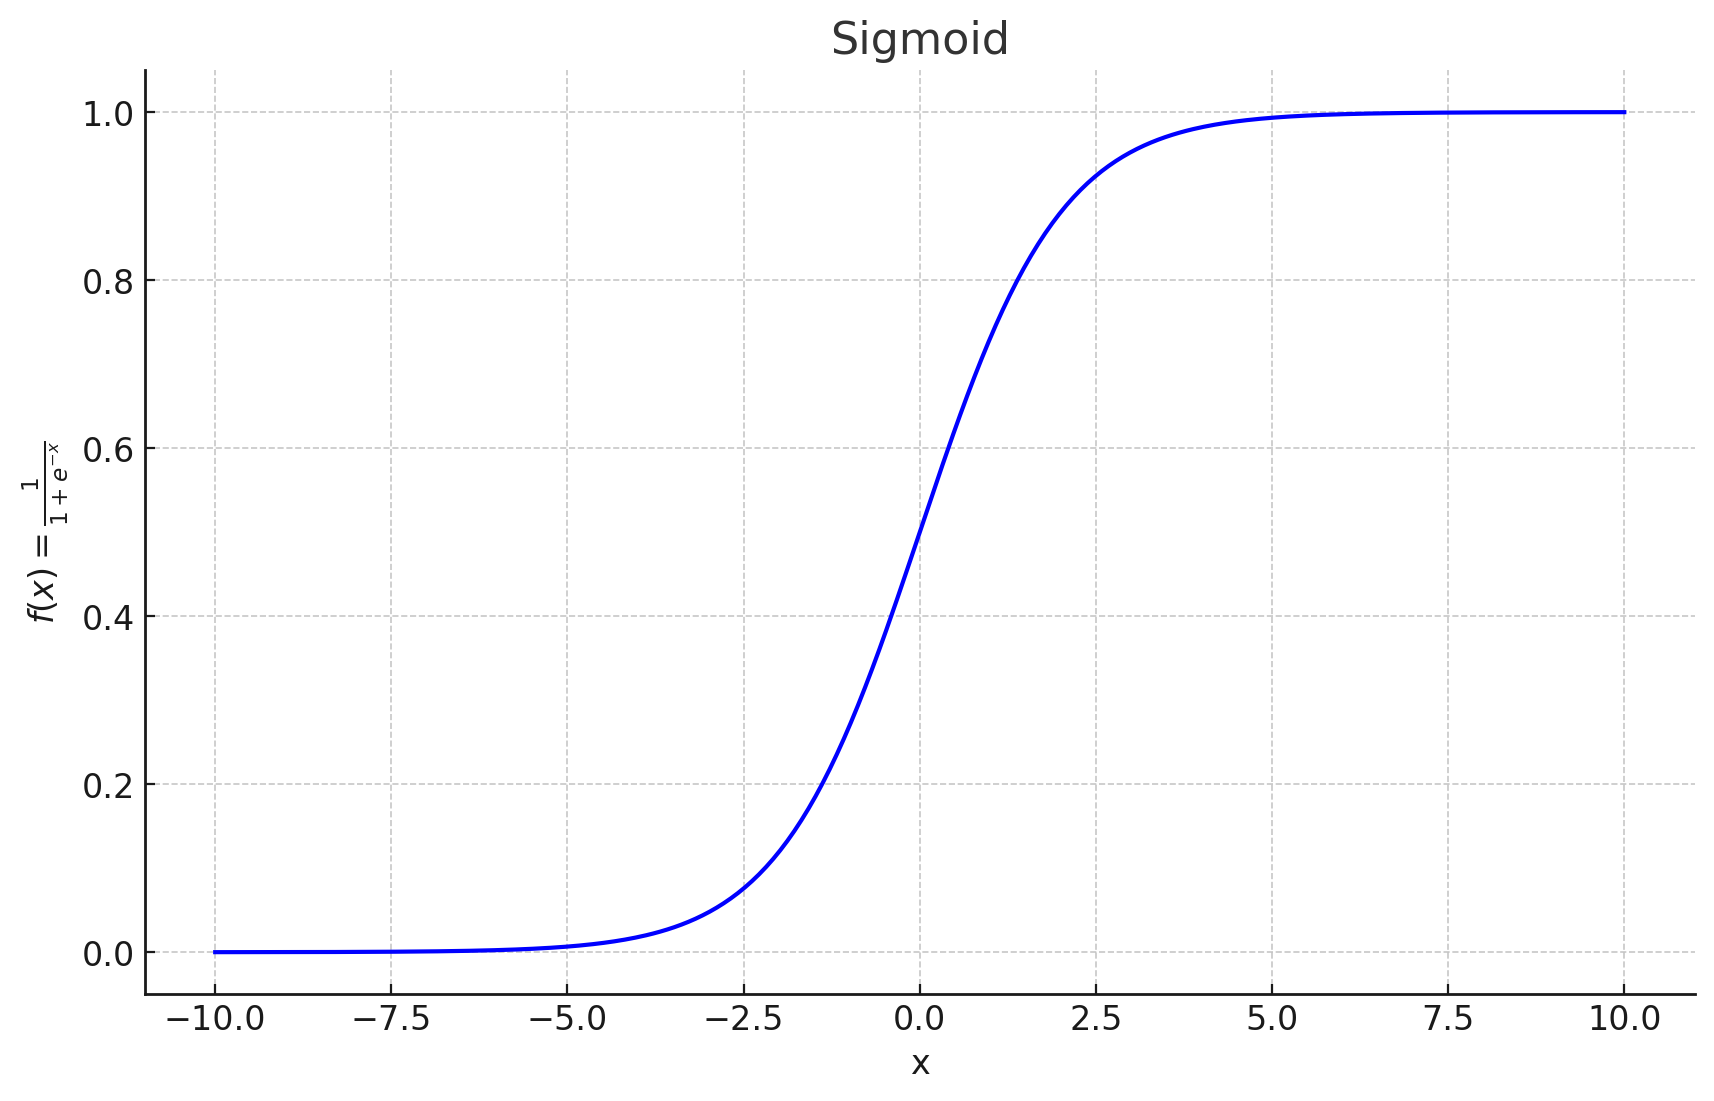
\includegraphics[width=0.25\textwidth]{images/sigmoid.png}
      \vspace{-2em}
    \end{figure}
  \item ReLU: $f(x) = \max(0, x)$
    \begin{figure}[H]
      \centering
      \vspace{-1em}
      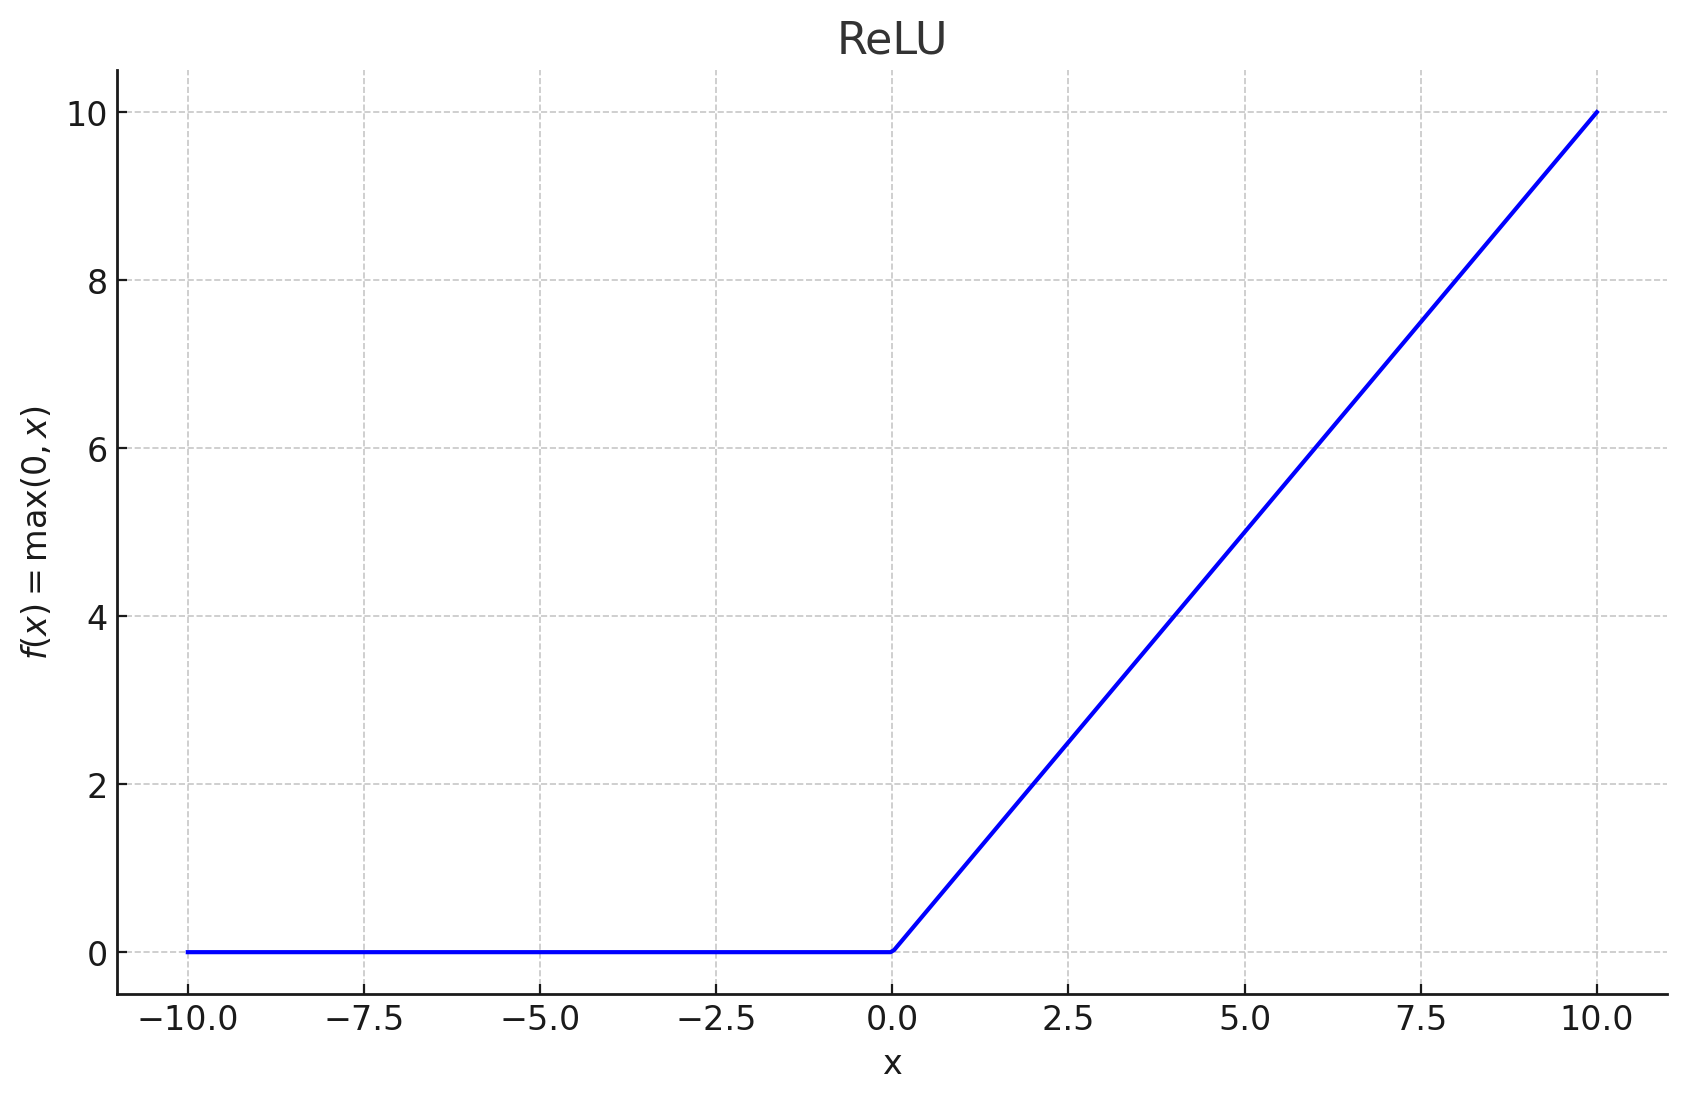
\includegraphics[width=0.25\textwidth]{images/relu.png}
      \vspace{-2em}
    \end{figure}
  \item Tanh: $f(x) = \frac{e^x - e^{-x}}{e^x + e^{-x}}$
    \begin{figure}[H]
      \centering
      \vspace{-1em}
      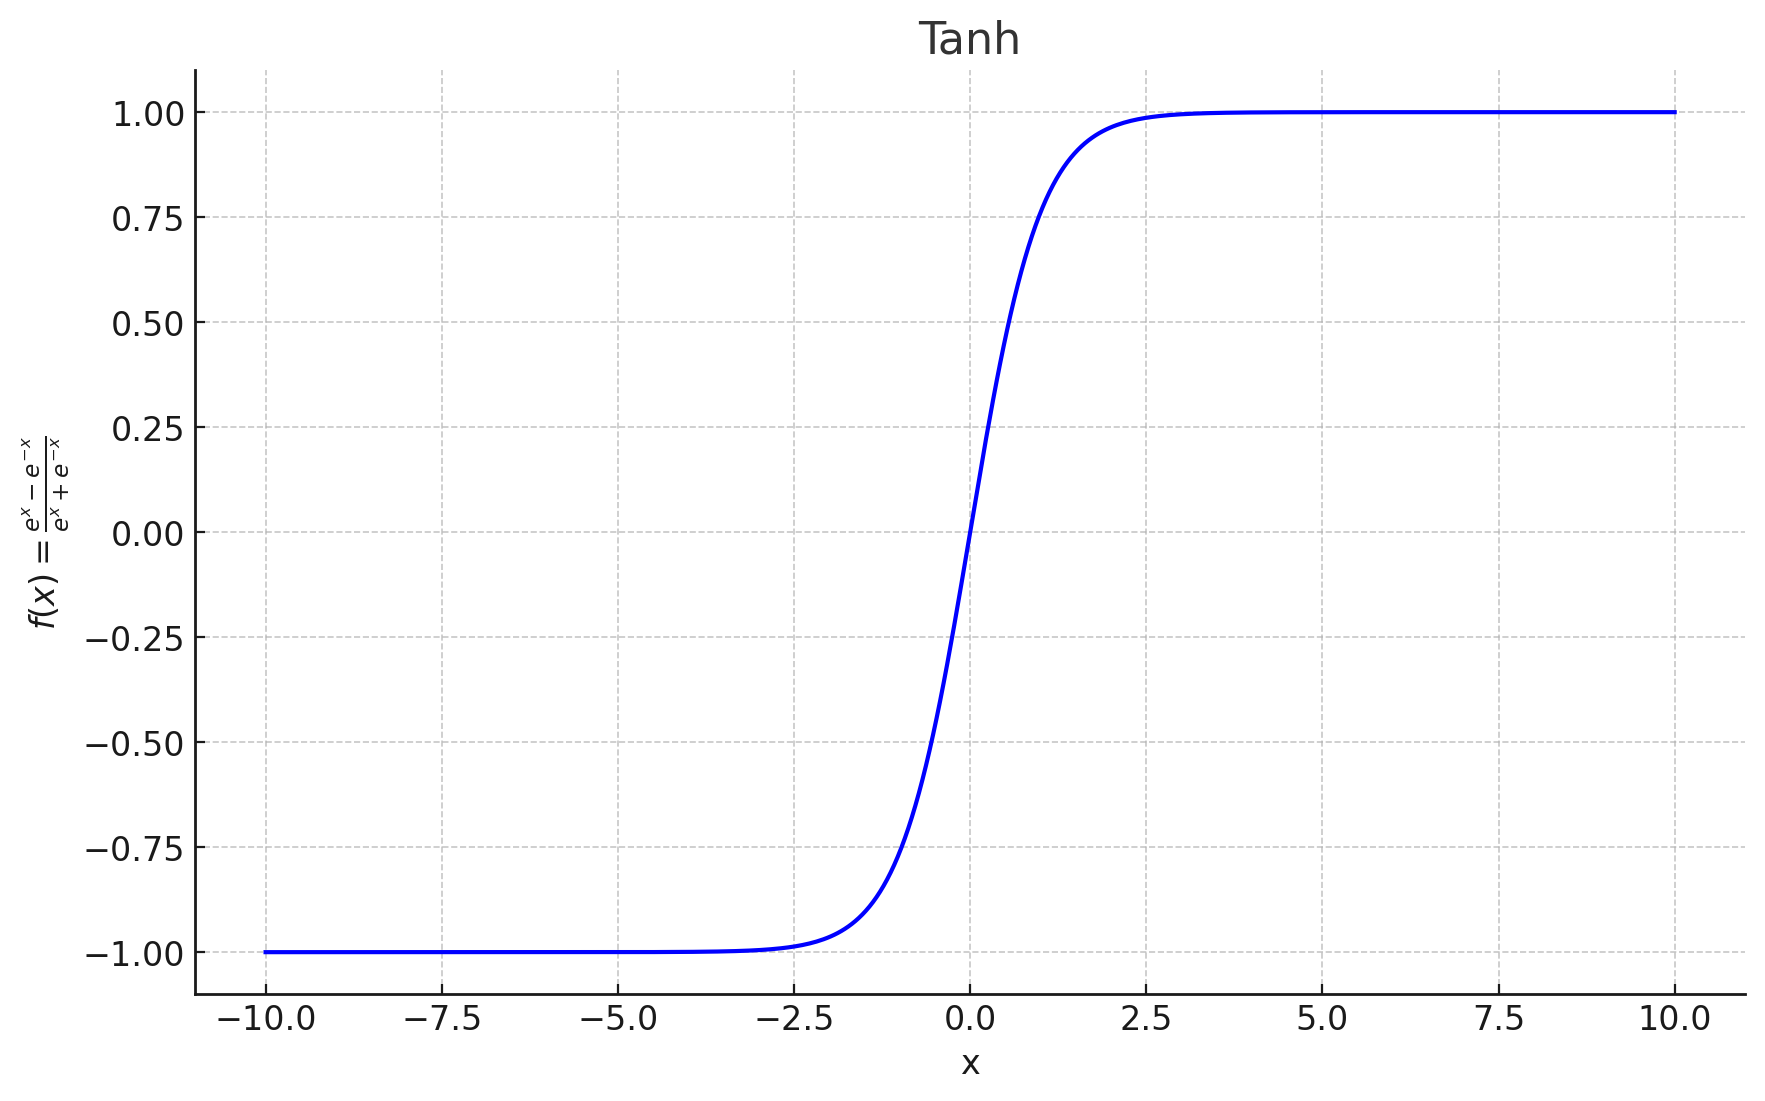
\includegraphics[width=0.25\textwidth]{images/tanh.png}
      \vspace{-2em}
    \end{figure}
  \item Softplus: $f(x) = \log(1 + e^x)$
    \begin{figure}[H]
      \centering
      \vspace{-1em}
      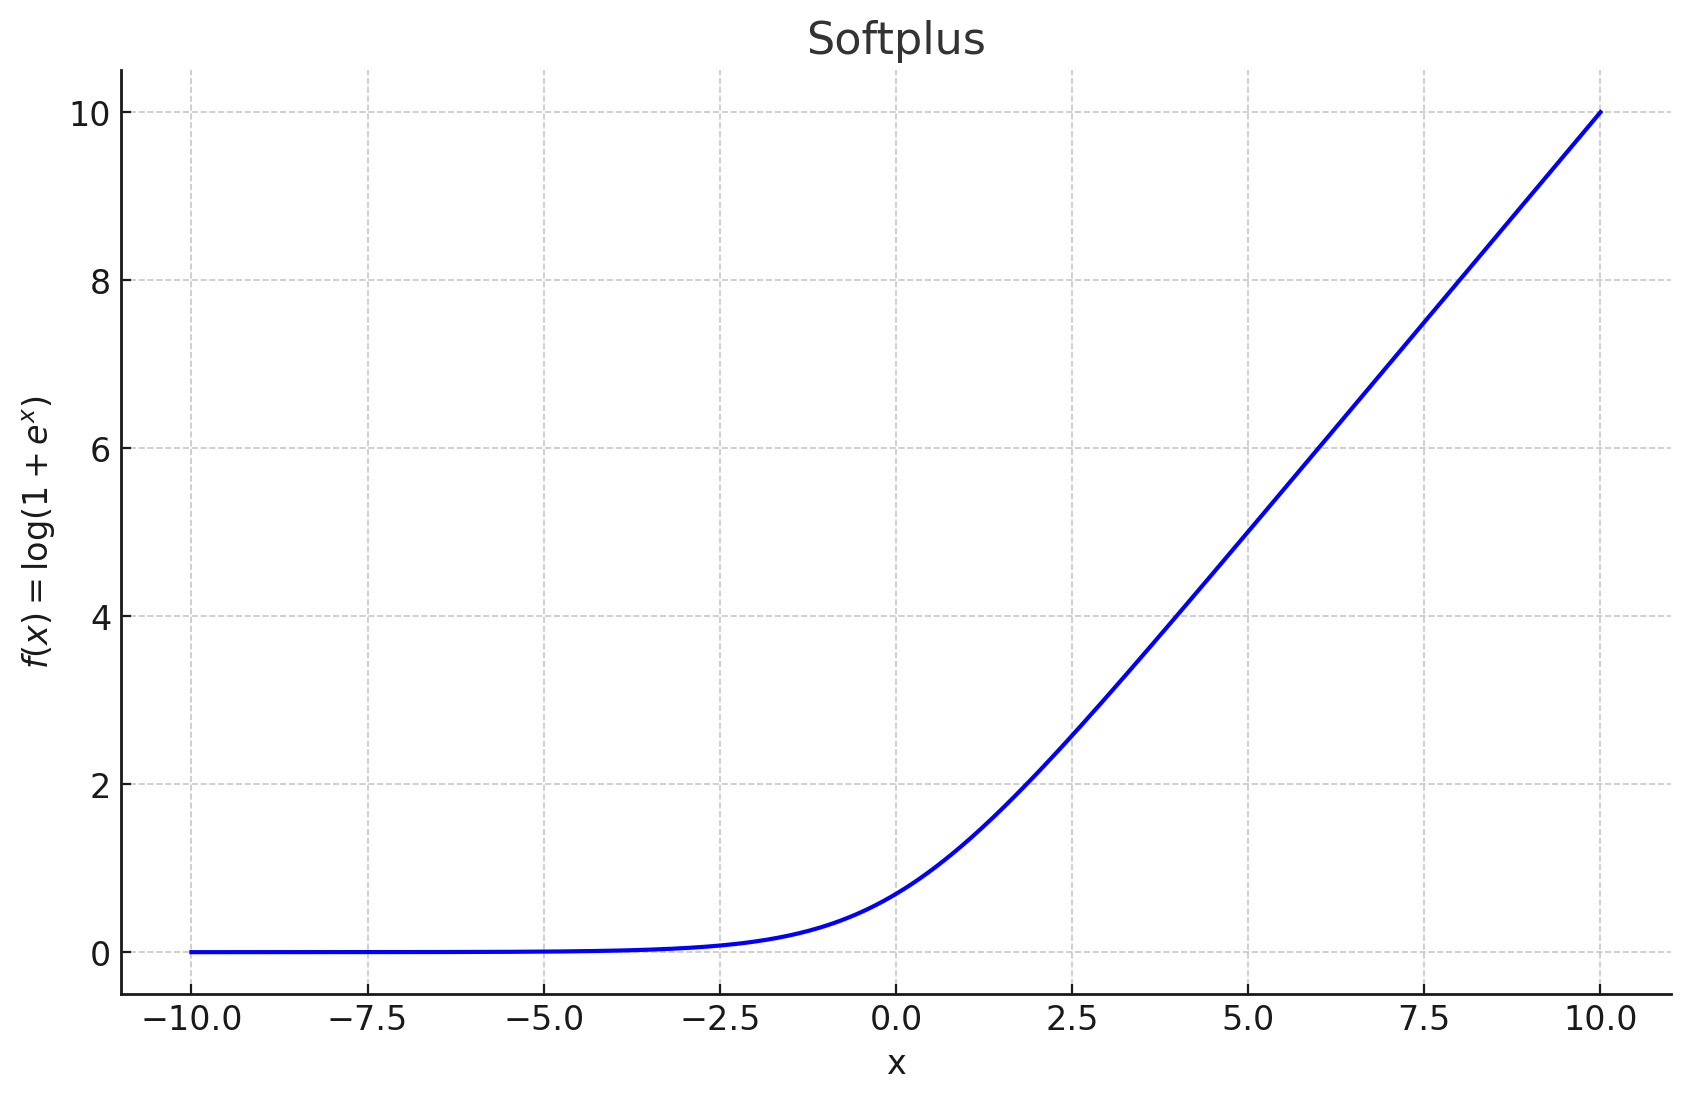
\includegraphics[width=0.25\textwidth]{images/softplus.png}
      \vspace{-2em}
    \end{figure}
  \item Approximated Sigmoid: $f(x) = \frac{x}{1 + |x|}$
    \begin{figure}[H]
      \centering
      \vspace{-1em}
      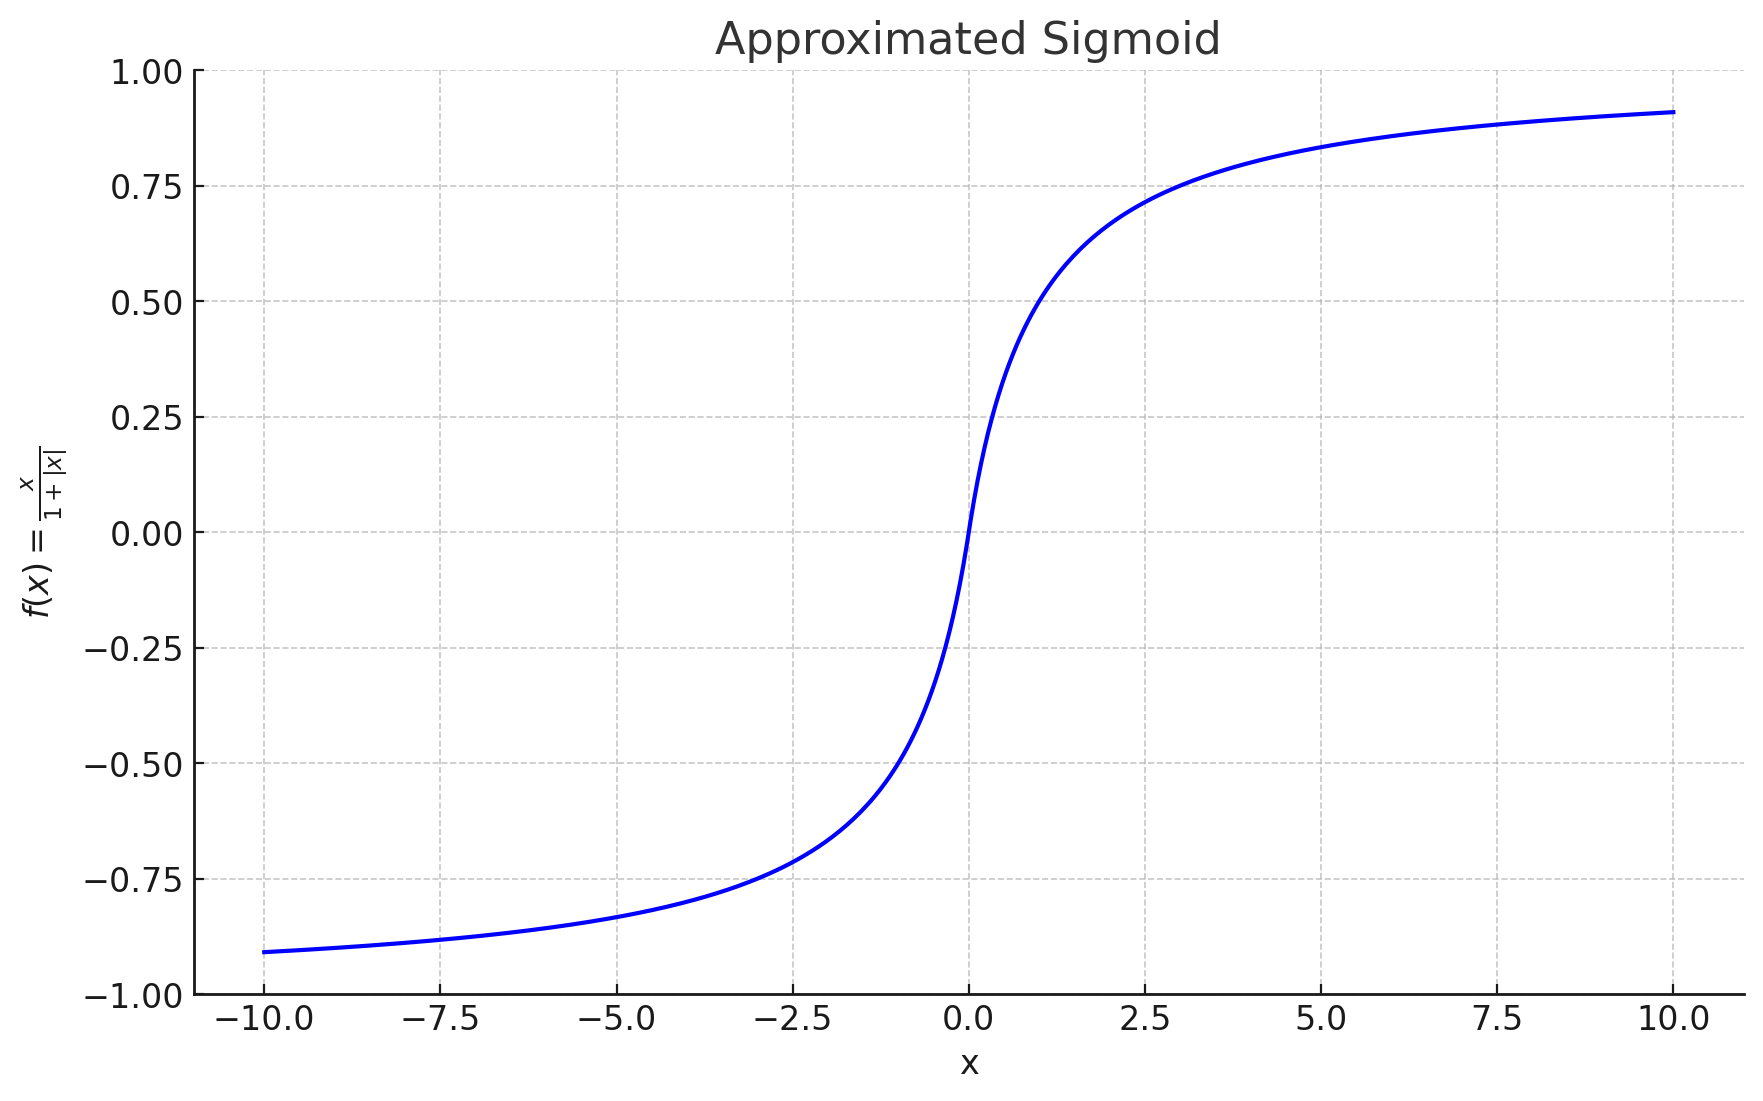
\includegraphics[width=0.25\textwidth]{images/approximated_sigmoid.png}
      \vspace{-2em}
    \end{figure}
\end{itemize}

\subsection*{Overfitting}

\textbf{Overfitting} occurs when a model learns the noise in the training data instead of the underlying pattern, leading to poor generalization on unseen data.

\textbf{Reasons for overfitting:} (i) limited training data, (ii) model complexity (excessive parameters compared to data) (iii) noisy or inaccurate data (iv) excessive training epochs without validation checks.

\textbf{Dealing with overfitting:}

\begin{itemize}
  \item \textbf{Early stopping:} When training complex models, often, training error decreases steadily while validation error begins to rise again. By stopping training at the lowest validation error point, we can avoid overfitting. \textbf{Additional cost:} maintaining copies of best model weights and validation error.
  \item \textbf{L2 Regularization:} Penalty term added to the loss function that discourages large weights. The loss function becomes $L(\mathbf{x}, \mathbf{y}) + \lambda ||\boldsymbol{\uptheta}||^2$, $\lambda \rightarrow$ hyperparameter controlling strength of regularization.

  \item \textbf{Dropout:} Similar to bagging. A set of sub-networks is obtained by randomly removing (\enquote{setting to zero}) \textbf{non-output} units from a base network. These sub-networks have shared weights. These are independently trained on a subset of the original training set, \textbf{sampled with replacement}.

    \begin{minipage}{\linewidth}
    \centering
    \includegraphics[width=0.7\textwidth]{images/dropout.png}
      \captionof{figure}{Some sub-networks have no inputs or paths joining them to the output; this problem is insignificant for large networks.}
  \end{minipage}
\end{itemize}

\subsection*{Optimization Algorithms}
Training neural networks takes a lot of time and computational resources. Optimization algorithms make this process more efficient.
\begin{itemize}
  \item \textbf{Mini-batch Gradient Descent:} Batch/Full-batch GD uses the entire training set to compute loss gradients, Stochastic GD uses one at a time. Mini-batch falls somewhere in between. Batch size is a hyperparameter. Choice of batch size is driven by:
    \begin{itemize}
      \item larger $\rightarrow$ more accurate gradient estimates 
      \item multi-core architectures/vector instruction sets are underutilized with very small batches (thus some absolute minimum is recommended)
      \item some kinds of hardware achieve better performance with specific sizes (GPUs notably do well with powers of 2; 32 to 256 are common, 16 is attempted for very large models)
    \end{itemize}
  \item \textbf{RMSProp:} Intuitively, RMSProp calculates a suitable learning rate for each parameter by scaling $\alpha$, th global learning rate proportional to a moving average of the inverse root sum of squares of the recent gradients. $\alpha$ itself remains unchanged.

    Normally during gradient descent, at each step, the weight update: $\boldsymbol{\uptheta} = \boldsymbol{\uptheta} + \Delta \boldsymbol{\uptheta}$, where $\Delta \boldsymbol{\uptheta} = -\alpha \nabla_{\boldsymbol{\uptheta}} J(\boldsymbol{\uptheta})$, where $\alpha$ is the learning rate.

    In RMSProp, we have a few additional steps:

    \begin{itemize}
      \item \textbf{Accumulate} the gradients in a moving average: $\mathbf{v}_t = \beta \mathbf{v}_{t-1} + (1 - \beta) \nabla_{\boldsymbol{\uptheta}} J(\boldsymbol{\uptheta})^2$, $\beta \rightarrow$ new hyperparameter ("how much of the gradient history to forget")
      \item \textbf{Scale} the learning rate for each parameter proportional to the inverse root of the accumulated gradient, $\mathbf{v}_t$: $\Delta \boldsymbol{\uptheta} = -\frac{\alpha}{\sqrt{\mathbf{v}_t + \epsilon}} \nabla_{\boldsymbol{\uptheta}} J(\boldsymbol{\uptheta})$, $\epsilon \rightarrow$ small constant to avoid division by zero.
    \end{itemize}

  \item \textbf{Adam:} Adam keeps track of two moving averages: (i) square gradients (as in RMSProp) (ii) gradients themselves.

    The second is essentially an incorporation of \textbf{momentum}. Thus, Adam can be thought of as a combination of RMSProp and momentum. \textbf{Key difference:} Adam includes \textbf{bias corrections} of both moments \textbf{to account for their initialization at zero}.

    Steps:

    \begin{itemize}
      \item \textbf{Accumulate} the gradients in a moving average: $\mathbf{m}_t = \beta_1 \mathbf{m}_{t-1} + (1 - \beta_1) \nabla_{\boldsymbol{\uptheta}} J(\boldsymbol{\uptheta})$, $\beta_1 \rightarrow$ hyperparameter controlling the decay rate of the first moment.
      \item \textbf{Accumulate} the square gradients in a moving average: $\mathbf{v}_t = \beta_2 \mathbf{v}_{t-1} + (1 - \beta_2) (\nabla_{\boldsymbol{\uptheta}} J(\boldsymbol{\uptheta}))^2$, $\beta_2 \rightarrow$ controls decay rate of second moment.
      \item Apply \textbf{bias corrections}: $\hat{\mathbf{m}}_t = \frac{\mathbf{m}_t}{1 - \beta_1^t}$, $\hat{\mathbf{v}}_t = \frac{\mathbf{v}_t}{1 - \beta_2^t}$.
      \item \textbf{Scale} the learning rate for each parameter, as in RMSProp: $\Delta \boldsymbol{\uptheta} = -\frac{\alpha}{\sqrt{\hat{\mathbf{v}}_t + \epsilon}} \hat{\mathbf{m}}_t$
    \end{itemize}

\end{itemize}

\subsection*{Batch Normalization}

Batch normalization is a method of \textbf{adaptive reparameterization}, motivated by the difficulty of training very deep models.

\begin{figure}[H]
  \centering
  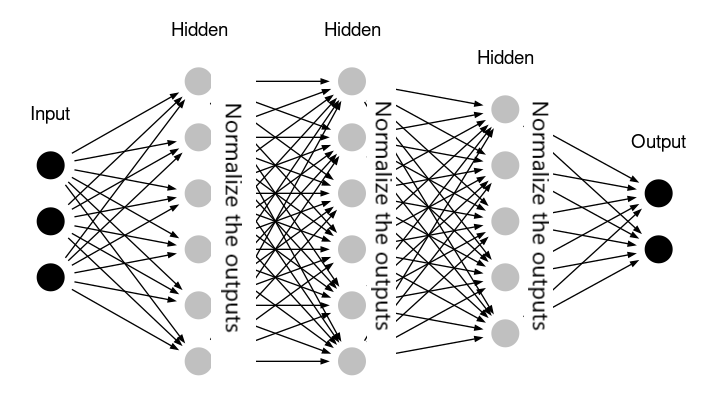
\includegraphics[width=0.375\textwidth]{images/batch_normalization.png}
\end{figure}

\begin{itemize}
  \item \textbf{Motivation:} Very deep models involve compositions of several functions/layers. The gradient tells us how to update each parameter, under the assumption that \textbf{all other parameters are fixed}.

    In practice, we update all the layers simultaneously. As we train, the distribution of each layer's inputs keeps changing.

    Batch normalization fixes each mini-batch to have \textbf{zero mean and unit variance}, which stabilizes the distribution of inputs to each layer.

  \item Let $\mathcal{B}$ be a mini-batch (size $m$) of activations of the layer (input or hidden) to normalize, arranged in matrix form where each row is the activations for each training example.

    To normalize $\mathcal{B}$, it is replaced with $\mathcal{B}' = \frac{\mathcal{B} - \mu}{\sigma}$

    $\mu = \frac{1}{m} \sum_{i=1}^m \mathcal{B}_i$, $\sigma = \sqrt{\delta + \frac{1}{m} \sum_{i=1}^m (\mathcal{B} - \mu)_i^2}$

  \item Normalizing the mean and standard deviation of a unit can \textbf{reduce the expressive power} of the network. As such, it is common to replace $\mathcal{B}$ with not plain $\mathcal{B}'$, but $\gamma \mathcal{B}' + \beta$, where $\gamma$ and $\beta$ are learnable parameters that scale and shift the normalized activations, allowing them to have \textbf{any mean and variance}.
\end{itemize}
